


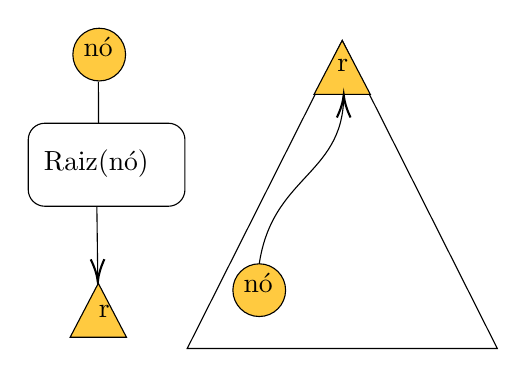
\begin{tikzpicture}[x=0.75pt,y=0.75pt,yscale=-1,xscale=1]
%uncomment if require: \path (0,300); %set diagram left start at 0, and has height of 300

%Rounded Rect [id:dp17006798515443122] 
\draw   (254.5,94.17) .. controls (254.5,89.75) and (258.08,86.17) .. (262.5,86.17) -- (322,86.17) .. controls (326.42,86.17) and (330,89.75) .. (330,94.17) -- (330,118.17) .. controls (330,122.59) and (326.42,126.17) .. (322,126.17) -- (262.5,126.17) .. controls (258.08,126.17) and (254.5,122.59) .. (254.5,118.17) -- cycle ;
%Straight Lines [id:da9040270232690516] 
\draw    (288.31,66.09) -- (288.38,85.97) ;
%Straight Lines [id:da5000031479986659] 
\draw    (287.56,126.15) -- (288,160.66) ;
\draw [shift={(288.03,162.66)}, rotate = 269.27] [color={rgb, 255:red, 0; green, 0; blue, 0 }  ][line width=0.75]    (10.93,-3.29) .. controls (6.95,-1.4) and (3.31,-0.3) .. (0,0) .. controls (3.31,0.3) and (6.95,1.4) .. (10.93,3.29)   ;
%Shape: Triangle [id:dp5248653828873222] 
\draw   (405.8,46.3) -- (480.5,194.7) -- (331.1,194.7) -- cycle ;
%Shape: Circle [id:dp3556155447935968] 
\draw  [fill={rgb, 255:red, 255; green, 202; blue, 64 }  ,fill opacity=1 ] (353.1,166.6) .. controls (353.1,159.59) and (358.79,153.9) .. (365.8,153.9) .. controls (372.81,153.9) and (378.5,159.59) .. (378.5,166.6) .. controls (378.5,173.61) and (372.81,179.3) .. (365.8,179.3) .. controls (358.79,179.3) and (353.1,173.61) .. (353.1,166.6) -- cycle ;
%Shape: Triangle [id:dp9990054770245029] 
\draw  [fill={rgb, 255:red, 255; green, 202; blue, 64 }  ,fill opacity=1 ] (405.76,46.3) -- (419.33,72.3) -- (392.19,72.3) -- cycle ;
%Curve Lines [id:da5640302566285083] 
\draw    (365.8,153.9) .. controls (372.12,111.69) and (405.48,111.33) .. (406.48,74.19) ;
\draw [shift={(406.5,72.47)}, rotate = 90] [color={rgb, 255:red, 0; green, 0; blue, 0 }  ][line width=0.75]    (10.93,-3.29) .. controls (6.95,-1.4) and (3.31,-0.3) .. (0,0) .. controls (3.31,0.3) and (6.95,1.4) .. (10.93,3.29)   ;
%Shape: Circle [id:dp8957416743815415] 
\draw  [fill={rgb, 255:red, 255; green, 202; blue, 64 }  ,fill opacity=1 ] (276,53.1) .. controls (276,46.09) and (281.69,40.4) .. (288.7,40.4) .. controls (295.71,40.4) and (301.4,46.09) .. (301.4,53.1) .. controls (301.4,60.11) and (295.71,65.8) .. (288.7,65.8) .. controls (281.69,65.8) and (276,60.11) .. (276,53.1) -- cycle ;
%Shape: Triangle [id:dp6360877133207615] 
\draw  [fill={rgb, 255:red, 255; green, 202; blue, 64 }  ,fill opacity=1 ] (288.26,163.3) -- (301.83,189.3) -- (274.69,189.3) -- cycle ;

% Text Node
\draw (260.74,97.72) node [anchor=north west][inner sep=0.75pt]   [align=left] {Raiz(nó)};
% Text Node
\draw (356.97,157.04) node [anchor=north west][inner sep=0.75pt]   [align=left] {nó};
% Text Node
\draw (402.2,54.12) node [anchor=north west][inner sep=0.75pt]   [align=left] {r};
% Text Node
\draw (279.87,43.54) node [anchor=north west][inner sep=0.75pt]   [align=left] {nó};
% Text Node
\draw (287.27,172.55) node [anchor=north west][inner sep=0.75pt]   [align=left] {r};


\end{tikzpicture}

